\vspace{-2mm}
\section{Experiments}
\label{sec:experiments}

\subsection{Experimental Setup}
\label{sec:experimental_setup}

\paragraph{Models and Datasets.}
We evaluate $\beta$-OPSD on the instruct-tuned Qwen3 model family, including
Qwen3-1.7B, Qwen3-4B, and Qwen3-8B. For training, we use the mathematical reasoning
subset of OpenThoughts. Each training example contains a problem $x$ and a ground-truth
solution, which we use as privileged information $c$ for the teacher branch. The student
generates solutions conditioned only on the problem $x$, while the privileged teacher can
condition on both $x$ and $c$ during training.

We evaluate on competition-level mathematical reasoning benchmarks, including
AIME 2024, AIME 2025, and HMMT 2025. These benchmarks require multi-step reasoning
and therefore test whether the method improves the quality of generated reasoning
trajectories rather than only local token imitation.

\paragraph{Baselines.}
We compare against three classes of baselines. First, we include the base model without
post-training. Second, we compare with supervised fine-tuning (SFT), which trains directly
on ground-truth solutions with the standard next-token prediction objective. Third, we
compare with vanilla on-policy self-distillation (OPSD), which distills directly toward the
privileged teacher using a local token-KL objective. In our notation, vanilla OPSD uses the
teacher endpoint as the target but does not use the scheduled interpolant curriculum or the
return-to-go credit-assignment estimator. We also compare with GRPO-style reinforcement
learning baselines, which optimize the student from sampled generations using
outcome-level rewards.

\paragraph{Implementation Details.}
For the main $\beta$-OPSD experiments, we use a bounded linear path for the teacher
weight rather than starting exactly at the student endpoint or ending exactly at the teacher
endpoint. Let
\begin{equation}
    s_k = \frac{k}{K-1},
    \qquad
    k=0,\ldots,K-1,
\end{equation}
be the normalized training progress. We define the practical teacher weight
\begin{equation}
    w_k
    =
    w_{\mathrm{start}}
    +
    \left(
    w_{\mathrm{end}}-w_{\mathrm{start}}
    \right)s_k,
    \label{eq:exp_weight_schedule}
\end{equation}
where $w_k=1/\beta_k$. Thus, $w_k$ is the teacher-side weight in the logit interpolant,
while $\beta_k$ is the corresponding regularization coefficient in the $\beta$-OPSD view.

At each update, we construct the interpolant target from a stop-gradient copy of the
current student and the privileged teacher. For a prefix $h_t=(x,y_{<t})$, we use
\begin{equation}
    \tilde p_{\beta_k}(\cdot\mid h_t,c)
    =
    \operatorname{softmax}
    \left(
    (1-w_k)z_{\bar{\theta}}(\cdot\mid h_t)
    +
    w_k z_T(\cdot\mid h_t,c)
    \right),
    \label{eq:exp_interpolant_target}
\end{equation}
where $\bar{\theta}=\operatorname{sg}(\theta)$ denotes a stop-gradient copy of the
current student. The token-level mismatch is
\begin{equation}
    \rho_t^{\beta_k}(y)
    =
    \log \pi_\theta(y_t\mid x,y_{<t})
    -
    \log \tilde p_{\beta_k}(y_t\mid x,y_{<t},c).
    \label{eq:exp_token_mismatch}
\end{equation}
We then compute the discounted return-to-go in Eq.~\ref{eq:slide_return_to_go} and the \ours{} loss in Eq.~\ref{eq:slide_loss}
\begin{equation}
    G_{t,\gamma}^{\beta_k}(y)
    =
    \sum_{s=t}^{T}
    \gamma^{s-t}
    \rho_s^{\beta_k}(y),
    \label{eq:exp_return_to_go}
\end{equation}
and optimize the practical $\beta$-OPSD loss
\begin{equation}
    \mathcal{L}_{\beta\text{-OPSD}}(\theta;y)
    =
    \frac{1}{T}
    \sum_{t=1}^{T}
    \operatorname{sg}
    \left(
    G_{t,\gamma}^{\beta_k}(y)
    \right)
    \log \pi_\theta(y_t\mid x,y_{<t}).
    \label{eq:exp_beta_opsd_loss}
\end{equation}

Unless otherwise specified, we use $w_{\mathrm{start}}=0.5$,
$w_{\mathrm{end}}=0.8$, $K=200$, and $\gamma=0.99$. These choices keep early targets
relatively close to the student while still exposing the model to stronger teacher guidance
later in training. All experiments are conducted on NVIDIA RTX A6000 or NVIDIA H200
GPUs with LoRA \citep{hu2022lora}. Additional training, generation, and evaluation details
are provided in Appendix~\ref{sec:exp_details}.

\begin{table*}[t]
\centering
\small
\caption{
Avg@12 results for Qwen3 models evaluated at the 100-step checkpoint from the default
200-step training schedule. Gains denote absolute differences of \ours{} relative to
Vanilla OPSD within the same model scale. For \ours{}, we report results under linear
schedules along the target path.
}
\label{tab:qwen3_results}
\setlength{\tabcolsep}{9pt}
\renewcommand{\arraystretch}{1.08}
\begin{tabular}{@{}lcccc@{}}
\toprule
Method
& AIME 2024
& AIME 2025
& HMMT 2025
& Average \\
\midrule

\multicolumn{5}{@{}l}{\textit{Qwen3-8B}} \\
\quad Base model
& 73.06
& 67.78
& 29.72
& 56.85 \\
\quad Vanilla OPSD
& 75.83
& 66.67
& \textbf{33.06}
& 58.52 \\
\quad SFT
& 72.78
& 64.72
& 30.83
& 56.11 \\
\quad GRPO
& 75.83
& 68.61
& 31.11
& 58.52 \\
\rowcolor{gray!12}
\quad \textbf{\oursbold{} (ours)}
& \textbf{78.33} \posgain{+2.50}
& \textbf{70.28} \posgain{+3.61}
& 31.94 \neggain{-1.12}
& \textbf{60.18} \posgain{+1.66} \\

\midrule

\multicolumn{5}{@{}l}{\textit{Qwen3-4B}} \\
\quad Base model
& \textbf{77.78}
& 64.17
& 29.44
& 57.13 \\
\quad Vanilla OPSD
& 75.00
& 65.00
& 28.33
& 56.11 \\
\quad SFT
& 23.61
& 19.72
& 10.56
& 17.96 \\
\quad GRPO
& 76.39
& 64.17
& 30.28
& 56.95 \\
\rowcolor{gray!12}
\quad \textbf{\oursbold{} (ours)}
& 73.89 \neggain{-1.11}
& \textbf{69.17} \posgain{+4.17}
& \textbf{30.56} \posgain{+2.23}
& \textbf{57.87} \posgain{+1.76} \\

\midrule

\multicolumn{5}{@{}l}{\textit{Qwen3-1.7B}} \\
\quad Base model
& 50.00
& 37.22
& 14.44
& 33.89 \\
\quad Vanilla OPSD
& 44.17
& 35.56
& 13.33
& 31.02 \\
\quad SFT
& 37.50
& 29.17
& 12.22
& 26.30 \\
\quad GRPO
& 48.33
& 38.61
& 15.00
& 33.98 \\
\rowcolor{gray!12}
\quad \textbf{\oursbold{} (ours)}
& \textbf{53.33} \posgain{+9.16}
& \textbf{40.83} \posgain{+5.27}
& \textbf{16.11} \posgain{+2.78}
& \textbf{36.76} \posgain{+5.74} \\

\bottomrule
\end{tabular}
\end{table*}
\begin{algorithm}[t]
\caption{\ours: Smooth Target Distillation Toward Logit Interpolants}
\label{alg:slide}
\begin{algorithmic}[1]
\Require Student $\pi_\theta$, privileged teacher $p_T$, dataset $\mathcal{D}$,
training budget $K$, schedule endpoints $w_{\mathrm{start}},w_{\mathrm{end}}$,
discount factor $\gamma$
\For{$k=0,\ldots,K-1$}
    \State Sample a minibatch $(x,c)\sim\mathcal{D}$
    \State Sample on-policy responses $y=(y_1,\ldots,y_T)\sim\pi_\theta(\cdot\mid x)$
    \State Set normalized progress $s_k=k/(K-1)$
    \State Set teacher weight $w_k$ by Eq.~\ref{eq:exp_weight_schedule} and $\beta_k=1/w_k$
    \State Set $\bar{\theta}\leftarrow \operatorname{sg}(\theta)$
    \State Construct interpolant targets $\tilde p_{\beta_k}(\cdot\mid h_t,c)$
    along the sampled prefixes using Eq.~\ref{eq:exp_interpolant_target}
    \State Compute token mismatches $\rho_t^{\beta_k}(y)$ using Eq.~\ref{eq:exp_token_mismatch}
    \State Compute discounted return-to-go weights $G_{t,\gamma}^{\beta_k}(y)$
    using Eq.~\ref{eq:exp_return_to_go}
    \State Minimize $\mathcal{L}_{\ours}(\theta;y)$ in Eq.~\ref{eq:exp_beta_opsd_loss}
    and update $\theta$
\EndFor
\end{algorithmic}
\end{algorithm}

\subsection{Results on Math Reasoning}
\label{sec:math_results}

Table~\ref{tab:qwen3_results} reports avg@12 performance for Qwen3 models evaluated
at the 100-step checkpoint from the default 200-step training schedule. Across all three
model scales, $\beta$-OPSD improves the overall average over Vanilla OPSD and achieves
the best average performance among all evaluated methods. The gains are most pronounced
for Qwen3-1.7B, where $\beta$-OPSD improves over Vanilla OPSD by $9.16$, $5.27$,
and $2.78$ points on AIME 2024, AIME 2025, and HMMT 2025, respectively, yielding a
$5.74$-point improvement in average performance.

The larger-scale results show that the method remains competitive as model size increases.
On Qwen3-4B and Qwen3-8B,
$\beta$-OPSD improves the overall average over Vanilla OPSD by $1.76$ and $1.66$
points, respectively. While it slightly underperforms Vanilla OPSD on some individual
benchmarks, such as AIME 2024 for Qwen3-4B and HMMT 2025 for Qwen3-8B, it gives
the strongest overall performance across the benchmark suite.

Compared with other post-training baselines, $\beta$-OPSD consistently outperforms SFT
across all model scales and achieves stronger performance than GRPO. Overall, these results support our central claim: replacing direct teacher imitation with
scheduled logit-interpolant targets provides a smoother and more effective distillation
objective. The advantage is especially clear for smaller models, where the student--teacher
distributional gap is larger, and remains competitive or stronger at larger
scales.

\subsection{Ablation Studies}
\label{sec:ablation_studies}

We conduct controlled ablations to isolate the contribution of each component of
$\beta$-OPSD. Unless otherwise specified, all variants use the same student, privileged
teacher, training data, optimization hyperparameters, training budget, and evaluation
protocol as the main experiments. We vary only the target distribution, credit-assignment
estimator, interpolant reference, or interpolation schedule under study. All ablations are
conducted with Qwen3-1.7B and report avg@12 on AIME 2024, AIME 2025, and HMMT 2025.

\subsubsection{Effect of Logit Interpolants}
\label{sec:ablation_logit_interpolants}

We first study whether the improvement of $\beta$-OPSD comes from the logit-interpolant
target or solely from the return-to-go credit-assignment estimator. To isolate the effect of
the target distribution, we apply the same return-to-go loss to two different distillation
targets.

The first variant, \emph{Teacher + Return-to-go}, distills directly toward the privileged
teacher. Its token-level log-ratio is
\begin{equation}
    \rho_t^{\mathrm{teach}}(y)
    =
    \log \pi_\theta(y_t\mid x,y_{<t})
    -
    \log p_T(y_t\mid x,y_{<t},c),
\end{equation}
with return-to-go $G_{t,\gamma}^{\mathrm{teach}}(y)=\sum_{s=t}^{T}\gamma^{s-t}\rho_s^{\mathrm{teach}}(y).$

The second variant uses the scheduled $\beta$-OPSD target. Its token-level log-ratio is 
\begin{equation}
    \rho_t^{\beta_k}(y)
    =
    \log \pi_\theta(y_t\mid x,y_{<t})
    -
    \log \tilde p_{\beta_k}(y_t\mid x,y_{<t},c),
\end{equation}
with return-to-go $G_{t,\gamma}^{\beta_k}(y)=\sum_{s=t}^{T}\gamma^{s-t}\rho_s^{\beta_k}(y).$

Both variants use student on-policy trajectories and identical return-to-go credit
assignment. Therefore, this comparison isolates the benefit of replacing the fixed teacher
target with the scheduled logit-interpolant target.

As shown in Table~\ref{tab:logit_interpolant_ablation}, the $\beta$-OPSD target
consistently outperforms direct teacher distillation, improving avg@12 by $6.03$ points on
AIME 2024, $5.30$ points on AIME 2025, and $1.67$ points on HMMT 2025. These gains
highlight the importance of a smooth transition in the target objective: rather than abruptly
projecting the student onto the teacher, the interpolant target reduces the student--target
gap and provides a more stable learning signal.

\begin{table}[t]
\centering
\small
\caption{
Effect of the distillation target. Both variants use the same return-to-go
estimator. We report avg@12 (\%); the best result in each column is bolded. For the \ours{} target, we report the result with $w_{\mathrm{start}}=0.5$ and $w_{\mathrm{end}}=0.8$.
}
\label{tab:logit_interpolant_ablation}
\begin{tabular}{lccc}
\toprule
Method
& AIME 2024
& AIME 2025
& HMMT 2025 \\
\midrule
Teacher + Return-to-go
& 47.30
& 35.53
& 14.44 \\
\textbf{\oursbold{} target}
& \textbf{53.33}
& \textbf{40.83}
& \textbf{16.11} \\
\bottomrule
\end{tabular}
\end{table}

\subsubsection{Effect of Return-to-go Credit Assignment}
\label{sec:ablation_lookahead_loss}

We next isolate the contribution of return-to-go credit assignment. Both variants use the
same logit-interpolant target $\tilde p_{\beta_k}$ and the same student-generated
trajectories, but differ in how the token-level signal is assigned.

The \emph{Local Token Gradient} variant uses only the instantaneous log-ratio:
\begin{equation}
    \widehat{g}_{\mathrm{local}}(y)
    =
    \sum_{t=1}^{T}
    \rho_t^{\beta_k}(y)
    \nabla_\theta
    \log \pi_\theta(y_t\mid x,y_{<t}).
    \label{eq:ablation_local_gradient}
\end{equation}
In contrast, the \emph{Return-to-go} variant uses the cumulative future mismatch:
\begin{equation}
    \widehat{g}_{\mathrm{RTG}}(y)
    =
    \sum_{t=1}^{T}
    G_{t,\gamma}^{\beta_k}(y)
    \nabla_\theta
    \log \pi_\theta(y_t\mid x,y_{<t}).
    \label{eq:ablation_rtg_gradient}
\end{equation}

As shown in Table~\ref{tab:lookahead_credit_ablation}, return-to-go credit assignment
consistently outperforms the local token-gradient objective. It improves avg@12 by
$1.12$ points on AIME 2024, $5.55$ points on AIME 2025, and $3.61$ points on
HMMT 2025. Since the two variants share the same target and sampling distribution, these
gains isolate the benefit of assigning earlier tokens credit for the future KL mismatch they
induce.

\begin{table}[t]
\centering
\small
\caption{
Effect of return-to-go credit assignment. Both variants use the same logit-interpolant
target with fixed schedules $w_{k}=\frac{1}{\beta_k}=0.5$. We report avg@12 (\%).
}
\label{tab:lookahead_credit_ablation}
\begin{tabular}{lccc}
\toprule
Method
& AIME 2024
& AIME 2025
& HMMT 2025 \\
\midrule
Local Token Gradient& 49.44
& 32.78
& 13.06 \\
\textbf{Return-to-go Gradient}
& \textbf{50.56}
& \textbf{38.33}
& \textbf{16.67} \\
\bottomrule
\end{tabular}
\end{table}


\subsubsection{Effect of Interpolant References}
\label{sec:ablation_interpolant_reference}

We ablate how the two endpoints of the logit interpolant are constructed. Let
$\theta_0$ denote the initial student parameters, let $\theta_k$ denote the student
parameters at training step $k$, and let
$\bar{\theta}_k=\operatorname{sg}(\theta_k)$ denote a stop-gradient copy of the current
student. In our self-distillation setting, the teacher branch uses the same model
architecture but additionally conditions on privileged information $c$.

We compare three reference choices. First, \emph{fixed student + fixed teacher} constructs
both endpoints from the initial model:
\begin{equation}
    \tilde p_{w}^{\mathrm{FF}}
    (\cdot\mid h_t,c)
    =
    \operatorname{softmax}
    \left(
    (1-w)z_{\theta_0}(\cdot\mid h_t)
    +
    w z_{\theta_0}(\cdot\mid h_t,c)
    \right).
    \label{eq:fixed_fixed_interpolant}
\end{equation}
Second, \emph{dynamic student + dynamic teacher} refreshes both endpoints from the
current model:
\begin{equation}
    \tilde p_{w}^{\mathrm{DD}}
    (\cdot\mid h_t,c)
    =
    \operatorname{softmax}
    \left(
    (1-w)z_{\bar{\theta}_k}(\cdot\mid h_t)
    +
    w z_{\bar{\theta}_k}(\cdot\mid h_t,c)
    \right).
    \label{eq:dynamic_dynamic_interpolant}
\end{equation}
Third, \emph{dynamic student + fixed teacher}, our default construction, uses the current
student as the student-side endpoint and a fixed privileged teacher as the teacher-side
endpoint:
\begin{equation}
    \tilde p_{w}^{\mathrm{DF}}
    (\cdot\mid h_t,c)
    =
    \operatorname{softmax}
    \left(
    (1-w)z_{\bar{\theta}_k}(\cdot\mid h_t)
    +
    w z_{\theta_0}(\cdot\mid h_t,c)
    \right).
    \label{eq:dynamic_fixed_interpolant}
\end{equation}

To isolate the effect of the interpolant references, we evaluate all three constructions using
the same return-to-go estimator and identical training settings. We keep the teacher weight
fixed at $w=0.5$, so that the two endpoints contribute equally to the target distribution.
As shown in Figure~\ref{fig:interpolant_reference_ablation}, the dynamic-student and
fixed-teacher construction performs best across all three benchmarks. These results suggest
that the interpolant benefits from tracking the evolving student distribution while retaining
a stable privileged teacher as its supervisory anchor.


\begin{figure}[t]
    \centering
    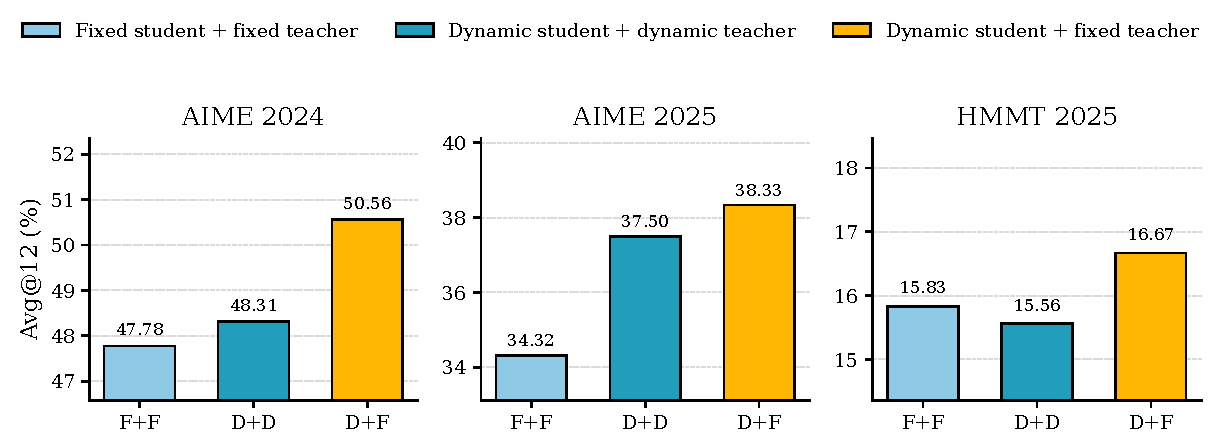
\includegraphics[width=\columnwidth]{figures/interpolant_reference_ablation.pdf}
    \caption{
    Effect of interpolant reference choices. All variants use the same return-to-go
    estimator and fixed teacher weight $w_k=1/\beta_k=0.5$. We report avg@12.
    Each subplot uses a benchmark-specific y-axis range to highlight relative differences.
    The dynamic student + fixed teacher construction performs best across all benchmarks.
    }
    \label{fig:interpolant_reference_ablation}
\end{figure}

\subsubsection{Effect of the Interpolation Schedule}
\label{sec:ablation_interpolation_schedule}

Finally, we study how the interpolation schedule affects performance. We focus on linear
schedules for the teacher weight $w_k=1/\beta_k$, varying the start and end values in
Eq.~\ref{eq:exp_weight_schedule}. We also include a fixed $w_k=0.5$ baseline.

As shown in Table~\ref{tab:interpolation_schedule_ablation}, the schedule influences
performance across benchmarks. The $0.5\rightarrow0.8$ schedule gives the strongest
overall result among the schedules considered here, while other schedules can be better on
individual benchmarks. This suggests that the strength and timing of teacher guidance are
important practical choices. Beyond the linear schedules studied here, nonlinear,
piecewise, or performance-adaptive schedules may further improve performance. Determining
whether an optimal schedule exists, and how it depends on model scale, training budget,
and task distribution, is an interesting direction for future work.

\begin{table}[t]
\centering
\small
\caption{
Effect of interpolation schedules. The notation $a\rightarrow b$ indicates that the teacher-weight endpoints $w_{\mathrm{start}}=a$ and $w_{\mathrm{end}}=b$ are using the schedule in Eq~\ref{eq:exp_weight_schedule}. We report avg@12 (\%).
}
\label{tab:interpolation_schedule_ablation}
\begin{tabular}{lccc}
\toprule
Schedule
& AIME 2024
& AIME 2025
& HMMT 2025 \\
\midrule
Fixed $0.5$
& 50.56
& 38.33
& \textbf{16.67} \\

Linear $0.2\rightarrow0.8$
& 51.39
& 37.50
& 16.39 \\

Linear $0.8\rightarrow0.2$
& 51.94
& 38.06
& 15.83 \\

Linear $0.5\rightarrow0.8$
& 53.33
& \textbf{40.83}
& 16.11 \\

Linear $0.8\rightarrow0.5$
& \textbf{54.72}
& 38.61
& 15.83 \\
\bottomrule
\end{tabular}
\end{table}

\begin{remark}
In addition to $\beta$-OPSD, which changes the distillation target through scheduled
logit interpolants, one can also construct guided rollouts by sampling from a mixture of the
student and the privileged teacher. This variant changes the trajectory distribution rather
than only the target distribution, and therefore requires importance correction. We provide
details and results in Appendix~\ref{app:proposal_mixture}.
\end{remark}